% SUPERSEDED by draft_v6.tex (2026-10-13). Historical draft only.
% The exclusive-cancellation claim, Proposition 1/2 guarantees, MASA citation,
% rollback-as-forgetting claim and universal-defense conclusion below are withdrawn.
% See PAIRED_AUDIT_MATH.md and REVISION_REPORT.md before reusing any claims.
% 초안 v5 — 학술 문체. 구성은 FLDetector(KDD'22)·FLAME(USENIX Sec'22) 의 전개를 따른다:
% 서론(배경·한계·제안·기여) → 관련 연구 → 위협 모델(공격자·방어자의 목표/능력/지식) → 제안 기법(개요·핵심 관찰·탐지 통계·판정·대응) → 분석 → 실험(설정·RQ 별 결과·민감도·비용) → 논의 및 한계 → 결론
% XeLaTeX + kotex. tectonic -o docs/paper docs/paper/draft_v5.tex
\documentclass[10pt,a4paper]{article}
\usepackage{kotex}
\IfFontExistsTF{Noto Sans CJK KR}{\setmainhangulfont{Noto Sans CJK KR}}{\setmainhangulfont{Malgun Gothic}}
\usepackage[margin=20mm]{geometry}
\usepackage{amsmath,amssymb,amsthm}
\usepackage{booktabs,array}
\usepackage{graphicx}
\usepackage{algorithm,algpseudocode}
\usepackage[colorlinks=true,linkcolor=blue,citecolor=blue,urlcolor=blue]{hyperref}
\usepackage{xcolor}
\newcommand{\todo}[1]{\textcolor{red}{[#1]}}
\newcommand{\method}{CCD}
\newtheorem{proposition}{명제}
\newtheorem{definition}{정의}
\graphicspath{{./}}

\title{연합 언러닝에서 삭제 요청으로 활성화되는 백도어의 학습 중 탐지:\\클라이언트 기여도의 상쇄 구조를 이용한 공모 식별}
\author{(저자)}
\date{초안 v5, 2026-10-13}

\begin{document}
\maketitle

\begin{abstract}
연합 언러닝(federated unlearning, FU)은 클라이언트의 삭제 요청에 따라 서버가 보관 중인 해당 클라이언트의 기여를 전역 모델에서 제거하는 절차이다. 최근 제안된 언러닝 활성화 백도어 공격(FUBA, BadFU)은 이 절차를 공격 경로로 전용한다. 일부 적대적 클라이언트(주입자)가 백도어를 주입하고 다른 적대적 클라이언트(억제자)가 동일 입력 영역에서 이를 상쇄함으로써 학습 종료 시점의 전역 모델을 정상으로 위장한 뒤, 억제자의 삭제 요청이 이행되는 순간 백도어가 활성화된다. 기존 비잔틴 내성 집계 및 백도어 탐지 기법은 개별 업데이트의 크기·방향 또는 업데이트 간 유사도만을 검사하므로, 서로 상쇄되도록 설계된 두 집단의 관계를 포착하지 못한다. 본 논문은 이러한 공격이 성립하기 위한 필요조건, 즉 특정 클래스에 대한 다수 클라이언트의 양(+)의 기여와 단일 클라이언트의 음(−)의 기여가 총합에서 상쇄되는 구조가 정상 학습에서는 발생하지 않는 관계적 불변량임을 보이고, 이를 학습 중에 검출하는 \method{}(Cancellation Coalition Detection)를 제안한다. \method{}는 라운드마다 참여 클라이언트의 업데이트가 공개 입력 집합 위에서 각 클래스의 로그 우도에 미치는 영향을 누적하고, 클래스별 상쇄 지수, 음의 기여 클라이언트의 강건 표준화 점수, 양의 기여 집합의 크기와 집중도로 공모 여부를 판정한다. 경보는 표적 클래스, 억제자, 주입자 집합, 복원 라운드를 함께 산출하며, 대응은 복원 라운드의 전역 모델에서 공모 집합을 배제하고 학습을 재개하는 것이다. FUBA의 논문 설정(클라이언트 20, 적대적 5, 100 라운드, 참여율 0.4, IID 및 non-IID 각 3 시드)에서 \method{}는 6개 궤적 모두에서 11--16 라운드에 경보를 발령하고 억제자와 주입자 4명을 정밀도·재현율 1.0으로 식별하였으며, 특정 클래스 데이터의 90\%를 보유한 정상 클라이언트를 오탐하지 않았다. 공모 집합을 배제한 재학습은 공격 성공률 0.5--0.6\%, 정확도 99\%를 달성하였다.
\end{abstract}

\section{서론}
연합학습(federated learning, FL)은 다수의 클라이언트가 원시 데이터를 공유하지 않고 모델 업데이트만을 교환하여 공동의 전역 모델을 학습하는 분산 학습 패러다임이다~\cite{krum}. GDPR의 삭제권과 같은 규제 요구에 따라, 특정 클라이언트의 기여를 학습된 모델에서 제거하는 연합 언러닝이 활발히 연구되고 있으며, FedEraser~\cite{federaser} 계열의 서버는 이를 위해 라운드별 클라이언트 업데이트를 보관한다.

이러한 보관과 제거 절차가 새로운 공격 표면이 된다. Zhang 등~\cite{zhang2023}, Liu 등~\cite{liu2024}, UBA-Inf~\cite{ubainf}, BadFU~\cite{badfu}, FUBA~\cite{fuba}는 공통적으로 다음 구조를 갖는다. 주입자(injector) 집합 $A$는 트리거 입력을 표적 클래스로 분류하게 하는 성분을 전역 모델에 주입하고, 억제자(suppressor) $S$는 동일 입력 영역에서 이를 상쇄하는 성분을 주입한다. 학습 종료 시점의 전역 모델 $\theta_T$는 정상으로 보이나(공격 성공률 3--8\%, 표~\ref{tab:attack}), 억제자의 삭제 요청에 따라 서버가 $U_S$를 제거하면 상쇄가 해제되어 백도어가 활성화된다(공격 성공률 46--93\%). 특히 서버가 삭제 요청을 정확하게 이행할수록 공격은 더 확실히 성공한다. 주입자를 포함한 채 처음부터 재학습하더라도 백도어가 재현된다($K=8$ 예비 실험, 30--44\%).

\paragraph{기존 기법의 한계.}
비잔틴 내성 집계 및 백도어 방어 기법은 개별 업데이트의 통계량(노름, Krum 거리~\cite{krum}, 서버 기준 모델과의 코사인 유사도~\cite{fltrust}, 출력층 에너지 분포~\cite{deepsight})이나 업데이트 간 유사도~\cite{foolsgold}, 라운드 간 일관성~\cite{fldetector}을 검사한다. 본 공격에서 억제자의 업데이트는 크기가 커서 크기 기반 기법에 포착되지만, 특정 클래스의 데이터를 집중 보유한 정상 클라이언트(이하 소유자) 역시 동일하게 포착되어 오탐이 발생한다(소유자 $z$ 점수 3.8--65, 표~\ref{tab:baselines}). 반면 주입자의 업데이트는 방향이 정상 집단의 중심에 위치하여(20명 중 평균 순위 18.5) 어떠한 단일 업데이트 기준으로도 식별되지 않는다. 언러닝 전용 탐지 기법(MASA~\cite{masa}, SubID~\cite{subid})은 삭제 요청자 한 명의 업데이트만을 검사하므로, 두 집단 간의 상쇄 관계를 원리적으로 관측할 수 없다.

\paragraph{핵심 관찰.}
공격 논문들은 잠복 상태를 ``한 손실 항이 다른 손실 항을 상쇄한다''는 서술에 그친다. 본 논문은 이를 동일 입력 영역에 대한 모순된 지도 신호의 평균화로 정식화한다. 전역 업데이트가 참여자 업데이트의 합이므로, 전역 모델의 출력 변화는 클라이언트별 기여로 선형 분해된다. 백도어가 잠복하기 위해서는 표적 클래스 $c^*$에 대한 기여의 총합이 0에 가까워야 하고, 삭제 후 활성화되기 위해서는 억제자의 기여 $|\Phi_S(c^*)|$가 주입자 기여의 합 $|\sum_{j\in A}\Phi_j(c^*)|$와 같은 크기로 커야 한다. 이는 다수의 양의 기여와 단일의 음의 기여가 상쇄되는 \emph{상쇄 연합}(cancellation coalition) 구조이며, 정직한 클라이언트의 손실 함수에는 타 클라이언트의 학습 결과를 되돌리는 항이 없으므로 정상 학습에서는 발생하지 않는다.

\paragraph{제안 기법.}
\method{}는 서버가 라운드마다 참여 클라이언트의 업데이트가 공개 입력 집합 위에서 각 클래스의 로그 우도 평균에 미치는 변화를 순전파로 측정하여 누적하고, 클래스별로 (i) 상쇄 지수, (ii) 최소 기여 클라이언트의 강건 표준화 점수, (iii) 유의한 양의 기여 집합의 크기, (iv) 양의 기여의 집중도를 계산하여 공모 여부를 판정한다. 경보는 표적 클래스, 억제자 후보, 주입자 후보 집합, 복원 라운드를 산출한다. 대응은 복원 라운드의 전역 모델에서 공모 집합을 배제하고 학습을 재개하는 것으로, 삭제 요청의 이행과 백도어 제거를 동시에 달성한다.

\paragraph{기여.}
\begin{enumerate}
\item 언러닝 활성화 백도어의 잠복 기제를 모순된 지도 신호의 평균화로 정식화하고, 공격 성립의 필요조건이 학습 중 관측 가능한 관계적 불변량(상쇄 연합)임을 보인다(\S\ref{sec:obs}, \S\ref{sec:analysis}).
\item 라벨·트리거·역할 정보 없이 라운드당 참여자 수만큼의 순전파로 상쇄 연합을 검출하고 표적 클래스·억제자·주입자·복원 라운드를 산출하는 학습 중 탐지 기법 \method{}를 제안한다(\S\ref{sec:method}).
\item 탐지 결과를 직접 활용하는 대응(복원 라운드 되돌림과 공모 집합 배제 후 학습 재개)을 제시하고, 학습 종료 후 요청에 대해서는 동일 통계량의 사후 계산으로 환원됨을 보인다(\S\ref{sec:response}).
\item FUBA 논문 설정의 6개 궤적에서 6/6 경보(11--16 라운드), 억제자·주입자 식별 정밀도·재현율 1.0, 소유자 오탐 0, 배제 재학습 후 공격 성공률 0.5--0.6\%를 달성하였으며, 9개 계열 36개 탐지 통계량과 동일 궤적에서 비교하였다(\S\ref{sec:eval}).
\end{enumerate}

\section{관련 연구}
\paragraph{연합 언러닝.} 서버는 $\theta_t=\theta_{t-1}+\frac{1}{|P_t|}\sum_{j\in P_t}u_j^t$로 전역 모델을 갱신하며($P_t$: 라운드 $t$ 참여자), 가중 업데이트 $U_j^t=u_j^t/|P_t|$를 보관한다. 삭제 요청 $k$에 대해 FedEraser~\cite{federaser}는 보관된 업데이트로 보정 재구성을, 감산 연산자는 $\theta_T-\rho\sum_tU_k^t$를, 재학습은 $k$를 제외한 전체 재학습을 수행한다. FedRecover~\cite{fedrecover}는 보관 업데이트를 이용한 오염 복구를 다룬다.

\paragraph{언러닝 활성화 백도어.} Zhang 등~\cite{zhang2023}은 오염 표본과 완화 표본(동일 트리거, 원래 라벨)을 함께 학습시킨 뒤 완화 표본의 삭제를 요청한다. Liu 등~\cite{liu2024}은 잠복 트리거를 언러닝으로 증폭한다. UBA-Inf~\cite{ubainf}는 영향 함수로 위장 표본을 최적화하며, 위장이 과도하면 백도어가 소실되고(vanishing) 부족하면 조기 노출된다(exposure)고 보고한다. 이는 상쇄의 크기가 정밀하게 균형을 이루어야 함을 의미한다. BadFU~\cite{badfu}는 전역 업데이트에 $p_1(\nabla L_{bd}+\nabla L_c)$가 포함되고 언러닝이 $\nabla L_c$를 제거하면 백도어 기울기가 온전히 작용함을 기술한다. FUBA~\cite{fuba}는 억제자를 적대적 방어자(Adv-defender)로 모델링하고 모델 일관성 손실로 전역 모델을 정상 모델에 근접시킨다. 이들 연구는 잠복 기제를 이론적 대상으로 다루지 않으며, 방어로는 요청 심사·사후 감시·차분 프라이버시를 언급하는 데 그친다.

\paragraph{FL 방어와 그 불변량.} Krum/Multi-Krum~\cite{krum}은 정상 기울기가 참 기울기 주변에 밀집한다는 가정, FLTrust~\cite{fltrust}는 서버 기준 업데이트와의 방향 일치, FLAME~\cite{flame}은 백도어 업데이트의 각도·크기 이탈, DeepSight~\cite{deepsight}는 오염 데이터의 낮은 이질성이 출력층에 남기는 흔적, FoolsGold~\cite{foolsgold}는 시빌 업데이트 간 유사성, FLDetector~\cite{fldetector}는 헤시안 기반 예측과의 라운드 간 일관성, BaFFLe~\cite{baffle}는 전역 모델의 클래스별 오류율 변화를 불변량으로 삼는다. 이들은 모두 단일 업데이트의 성질 또는 업데이트 간 유사성에 기반하며, 업데이트들이 서로 상쇄되는 관계를 불변량으로 두는 기법은 없다.

\paragraph{상쇄 현상의 이론적 틀.} 영향 함수~\cite{koh2017}, 협력 게임의 상호작용 지수~\cite{grabisch}, 과제 산술~\cite{ilharco}(과제 벡터의 부정이 망각에 대응), 다중 과제 학습의 기울기 충돌~\cite{pcgrad}이 관련된다. 본 논문은 ``연합 전체는 더미(dummy)이나 구성원은 더미가 아닌'' 협력 게임의 개념을 불변량의 명명에 차용하고, 신경 접선 커널(NTK) 선형화~\cite{hayase2022}를 기제 설명과 측정량의 정당화에 사용한다. 매개변수 공간에서의 쌍별 코사인 유사도 및 부호 충돌은 본 설정에서 억제자--주입자($+0.56$)와 억제자--정상($+0.60$)을 구분하지 못하였으므로 통계량으로 채택하지 않는다(R-005).

\section{위협 모델}\label{sec:threat}
\paragraph{시스템.} $K$개 클라이언트가 $T$ 라운드 동안 참여율 $p$로 FedAvg 학습을 수행한다. 서버는 각 라운드의 전역 모델 $\theta_{t-1}$, 참여자 집합 $P_t$, 업데이트 $u_j^t$를 보관한다(FU 서버의 전제). 서버는 라벨이 없는 공개 입력 집합 $X_p$($|X_p|=500$, 시험 분포)를 보유한다.
\paragraph{공격자.} 적대적 집합 $M\subset[K]$, $|M|<K/2$(논문 설정 5/20). $M$은 주입자 $A$와 억제자 $S$로 구성된다. 공격자의 목표는 (i) 학습 중 전역 모델이 트리거 입력에서 정상으로 동작하고(잠복), (ii) $S$의 삭제 요청이 이행된 후 트리거 입력이 표적 클래스 $c^*$로 분류되는 것(활성화)이다. 공격자는 자신의 데이터·손실·업데이트를 임의로 구성할 수 있으며(FUBA의 적대적 방어자 학습 포함), 백도어는 단일 표적 클래스를 갖는다(다중 표적은 \S\ref{sec:limit}).
\paragraph{정상 클라이언트.} 자신의 데이터로 정직하게 학습한다. 데이터 분포는 IID 또는 한 클라이언트가 한 클래스의 90\%를 보유하는 non-IID(소유자 조건)이다. 정상 클라이언트도 삭제를 요청할 수 있으며, 서버는 요청자의 의도를 판정하지 않는다.
\paragraph{방어자.} 서버는 트리거, 표적 클래스, 클라이언트의 역할, 적대적 클라이언트의 수를 알지 못한다. 방어 목표는 (G1) 삭제 요청 이전에 상쇄 연합을 검출하여 표적·억제자·주입자를 식별하고, (G2) 소유자를 포함한 정상 클라이언트를 배제하지 않으며, (G3) 삭제 요청을 이행하면서 백도어를 제거하고, (G4) 라벨·트리거·역할 정보와 추가 모델 생성 없이 라운드당 순전파만으로 동작하는 것이다.

\section{핵심 관찰: 모순된 지도 신호의 평균화와 상쇄 연합}\label{sec:obs}
\paragraph{선형 분해.} $f_c(x;\theta)$를 입력 $x$에 대한 클래스 $c$의 로그 우도라 하자. 라운드 $t$에서 참여자 $j$의 가중 업데이트 $U_j^t$가 공개 입력 $x$의 클래스 $c$에 미치는 1차 변화는 $\langle U_j^t,\nabla_\theta f_c(x;\theta_{t-1})\rangle$이며, 전역 업데이트에 의한 변화는 이들의 합이다. 이는 경험적 NTK 선형화의 클라이언트별 분해에 해당하며, 유한차분 $f_c(x;\theta_{t-1}+U_j^t)-f_c(x;\theta_{t-1})$는 순전파 한 번으로 그 비선형 값을 제공한다.

\begin{definition}[클래스별 누적 기여도]
클라이언트 $j$의 클래스 $c$에 대한 누적 기여도는
\begin{equation}
\Phi_j(c)=\sum_{t:\,j\in P_t}\ \operatorname{mean}_{x\in X_p}\big[f_c(x;\theta_{t-1}+U_j^t)-f_c(x;\theta_{t-1})\big].
\label{eq:phi}
\end{equation}
\end{definition}
정상 학습에서 $\Phi_j(c)$는 $j$의 데이터가 클래스 $c$의 학습에 기여한 정도이다. IID 분포에서는 클라이언트 간에 유사하고, 소유자는 자신의 클래스에서 큰 양의 값을 갖는다.

\paragraph{잠복의 필요조건.} 트리거 입력 집합 $X^*$ 위에서 성립하는 상쇄 조건 $J_{X^*}(U_S+\sum_{j\in A}U_j)\approx0$이 공개 입력 $X_p$로 전파되면(FUBA의 일관성 손실은 전역 모델 전체를 정상 모델 쪽으로 되돌리므로 전파가 관측된다, R-012), 누적 기여도에는
\begin{equation}
\Phi_S(c^*)\approx-\sum_{j\in A}\Phi_j(c^*),\qquad |\Phi_S(c^*)|\gg\max_{j\notin M}|\Phi_j(c^*)|
\end{equation}
가 남는다. 즉 클래스 $c^*$에서 (i) 기여도의 총합은 0에 가깝고, (ii) 개별 기여도는 크며, (iii) 음의 기여는 단일 클라이언트에 집중되고, (iv) 양의 기여는 복수의 클라이언트에 분산된다. 이 네 조건을 동시에 만족하는 클래스를 \emph{상쇄 연합이 존재하는 클래스}라 한다.

\paragraph{실측(R-012, 그림~\ref{fig:push}).} 논문 설정 6개 궤적의 학습 종료 시점에서 클래스 8의 누적 기여도는 억제자 $-29.7\ldots-39.4$(6/6 최솟값), 주입자 각 $+3.3\ldots+16.3$, 정상 $-3.9\ldots+4.9$, 소유자 $+0.2\ldots+3.8$이며, 총합의 크기는 개별 크기 합의 7--16\%였다.
\begin{figure}[t]\centering
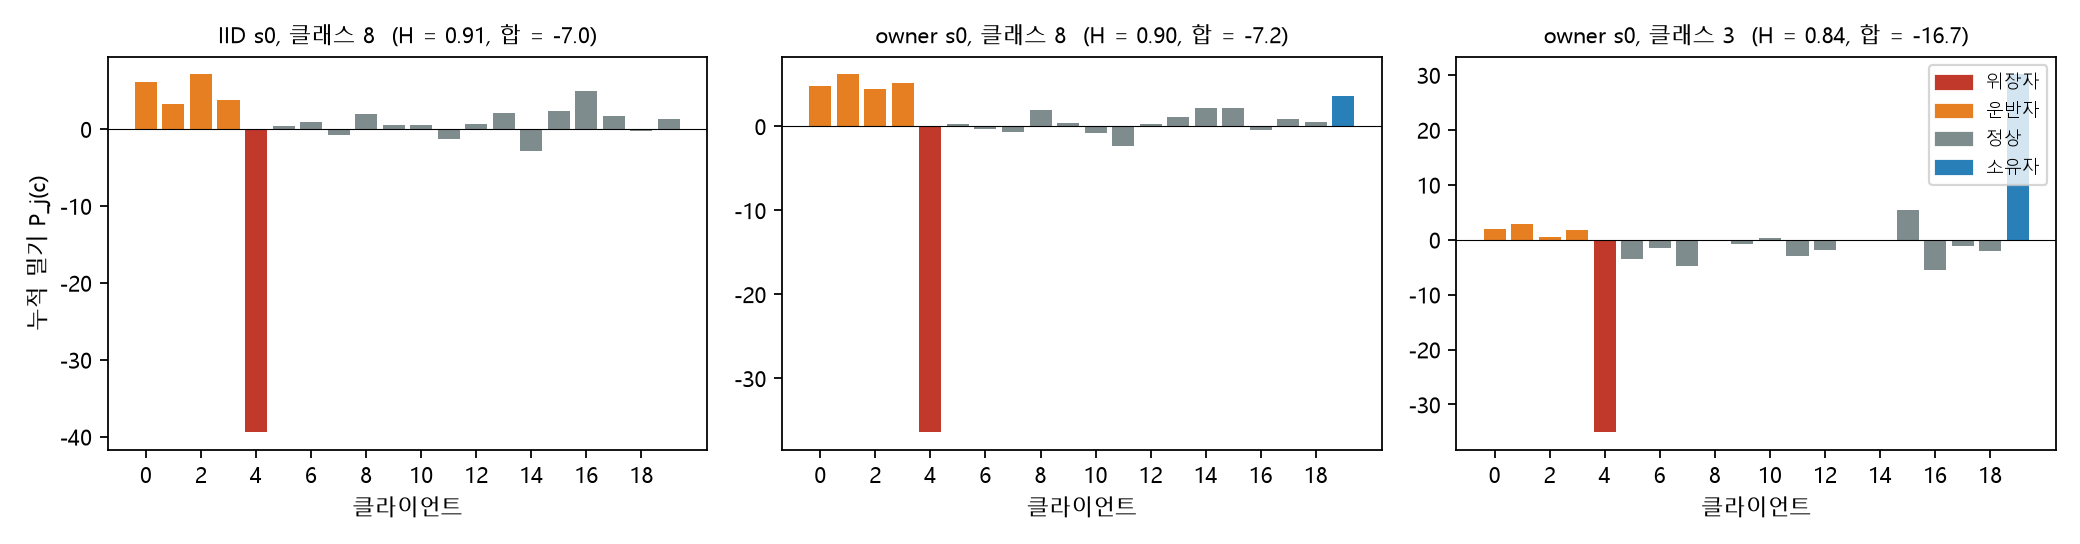
\includegraphics[width=\linewidth]{fig_push_bar.png}
\caption{학습 종료 시점의 클래스별 누적 기여도 $\Phi_j(c)$. 좌·중: 표적 클래스 8---주입자 4명(주황)의 양의 기여를 억제자(적색)가 단독으로 상쇄한다($H$ 0.91/0.90). 우: non-IID 조건의 소유 클래스 3---소유자(청색) 1명의 양의 기여를 억제자가 상쇄한다($H$ 0.84). 음의 기여 주체는 동일하나 양의 기여 집합의 크기가 다르다.}
\label{fig:push}
\end{figure}

\paragraph{정상 학습에서 부재하는 이유.} 정직한 클라이언트의 업데이트는 자신의 데이터에 대한 손실을 감소시킬 뿐이며, 타 클라이언트가 학습시킨 내용을 되돌리는 항을 포함하지 않는다. 따라서 IID에서는 기여도가 동일 부호로 누적되어 총합이 크고, non-IID에서는 소유자 1명의 큰 양의 기여에 대해 이를 상쇄하는 음의 기여가 존재하지 않는다. ``단일 클라이언트의 큰 음의 기여가 복수 클라이언트의 양의 기여 합과 일치''하는 구조는 데이터 분포의 차이로는 생성되지 않는다.

\paragraph{소유자와의 구분.} non-IID 조건에서 억제자는 표적 클래스뿐 아니라 소유자의 클래스 3도 상쇄한다(소유자 $+30$, 억제자 $-35$). 전역 모델의 변화 전체를 되돌리기 때문이다. 따라서 클래스 3 역시 조건 (i)--(iii)을 만족한다. 구분은 조건 (iv)에서 이루어진다. 클래스 8의 양의 기여는 주입자 4명에 분산되어 있으나(최대 1인 점유율 0.31--0.54), 클래스 3의 양의 기여는 소유자 1명에 집중된다(점유율 $>0.6$). 양의 기여가 복수 주체에 분산된 경우만을 공모로 판정하고, 단일 주체에 집중된 경우는 정상적인 데이터 편중으로 간주하여 개입하지 않는다.

\section{제안 기법: \method{}}\label{sec:method}
\subsection{개요}
\method{}는 학습 중 서버에서 동작하며, 라운드마다 (1) 참여자별 클래스별 기여도를 누적하고, (2) 클래스별 상쇄 통계량을 계산하며, (3) 판정 규칙으로 공모 클래스를 식별하고, (4) 지속성 조건을 만족하면 경보와 함께 표적 클래스·억제자·주입자 집합·복원 라운드를 산출한다. 대응은 \S\ref{sec:response}에 기술한다.

\subsection{탐지 통계량}
라운드 $t$ 종료 후 누적 기여도 행렬 $\Phi\in\mathbb{R}^{K\times C}$에 대해 클래스 $c$마다 다음을 계산한다.
\begin{align}
H(c)&=1-\Big|\sum_j\Phi_j(c)\Big|\Big/\sum_j|\Phi_j(c)| &&\text{(상쇄 지수)}\\
z_j(c)&=\frac{\Phi_j(c)-\operatorname{median}_i\Phi_i(c)}{\operatorname{MAD}_i\Phi_i(c)},\qquad s(c)=\arg\min_j\Phi_j(c) &&\text{(강건 표준화 점수, 최소 기여 클라이언트)}\\
\mathcal{P}(c)&=\{j\neq s(c): z_j(c)>\kappa\} &&\text{(유의한 양의 기여 집합)}\\
\rho(c)&=\max_{j\in\mathcal{P}(c)}\Phi_j(c)\Big/\sum_{j\in\mathcal{P}(c)}\Phi_j(c) &&\text{(양의 기여 집중도)}
\end{align}
상쇄 지수 $H(c)$는 기여도가 모두 동일 부호이면 0, 완전히 상쇄되면 1이다. 표준화에는 영분포를 동일 클래스의 다른 클라이언트들로 두는 MAD 기반 강건 점수를 사용한다(MASA~\cite{masa}, FLAME~\cite{flame}과 동일한 형식). 누적 참여 횟수가 $n_{\min}$ 미만인 클라이언트는 후보에서 제외한다(참여율 $<1$에서의 초기 결측 처리).

\subsection{판정 규칙}
클래스 $c$는 다음을 모두 만족할 때 \textbf{공모 클래스}로 판정한다.
\begin{equation}
H(c)\ge h_0\ \wedge\ z_{s(c)}(c)\le-\tau\ \wedge\ |\mathcal{P}(c)|\ge m\ \wedge\ \rho(c)\le\rho_0.
\label{eq:rule}
\end{equation}
앞의 두 조건을 만족하되 $|\mathcal{P}(c)|=1$ 또는 $\rho(c)>\rho_0$이면 \textbf{편중 클래스}(소유자형)로 분류하고 개입하지 않는다. $\mathcal{P}(c)=\emptyset$이면 \textbf{단독 음의 기여}로 기록만 한다(억제자는 전역 모델의 변화 전체를 되돌리므로 비표적 클래스에서도 발생한다). 동일 클래스가 $r$ 라운드 연속 공모로 판정되면 \textbf{경보}를 발령한다. 판정은 $t\ge t_0$부터 모든 클래스에 대해 수행한다. 고정값은 $h_0=0.8$, $\tau=3$, $\kappa=2$, $m=2$, $\rho_0=0.6$, $r=3$, $t_0=5$, $n_{\min}=2$이며, 민감도는 \S\ref{sec:sens}에서 분석한다.

\subsection{경보의 산출물}
표적 클래스 $c^*$, 억제자 후보 $s(c^*)$, 주입자 후보 집합(연속 판정 기간 동안 $\mathcal{P}(c^*)$에 속한 클라이언트의 합집합), 복원 라운드 $t_{\mathrm{back}}=\max\{t'<t_{\mathrm{alarm}}: H_{t'}(c^*)<h_0\}$.

\subsection{대응}\label{sec:response}
공모 집합 $\mathcal{C}=\{s(c^*)\}\cup\mathcal{P}(c^*)$에 대해, 전역 모델을 $\theta_{t_{\mathrm{back}}}$로 되돌리고 $\mathcal{C}$를 배제한 채 잔여 $T-t_{\mathrm{back}}$ 라운드의 학습을 재개한다. 되돌림은 공모가 주입되기 시작한 구간을 폐기하고, 배제는 재주입을 차단한다. 억제자의 삭제 요청은 이로써 이행되며, 주입자의 기여는 정당성이 없으므로 제거된다. 학습 종료 후에 삭제 요청이 도착하는 경우, 보관된 $\{U_j^t\}$에 대해 식~(\ref{eq:phi})--(\ref{eq:rule})을 사후 계산하면 동일한 판정이 얻어지며, 공모 집합을 배제한 재학습으로 요청을 이행한다. 즉 요청 시점 방어는 별도의 절차가 아니라 동일 통계량의 사후 적용이다.

\subsection{복잡도}
라운드당 $(|P_t|+1)$회의 순전파(공개 입력 500장)가 소요되며, 역전파·모델 생성·라벨·트리거 정보는 필요하지 않다. 대응의 비용은 $T-t_{\mathrm{back}}$ 라운드의 학습이다.

\begin{algorithm}[t]
\caption{\method{}: 학습 중 상쇄 연합 탐지}
\begin{algorithmic}[1]
\Require 라운드별 $(\theta_{t-1},P_t,\{U_j^t\})$, 공개 입력 $X_p$, 매개변수 $h_0,\tau,\kappa,m,\rho_0,r,t_0$
\State $\Phi\gets0_{K\times C}$; $\mathrm{streak}\gets0_C$
\For{$t=1,\dots,T$}
  \State $L_0\gets\operatorname{mean}_{x\in X_p}f(x;\theta_{t-1})$
  \For{$j\in P_t$} $\Phi_j\gets\Phi_j+\operatorname{mean}_{x\in X_p}f(x;\theta_{t-1}+U_j^t)-L_0$ \EndFor
  \If{$t<t_0$} \textbf{continue} \EndIf
  \For{$c=1,\dots,C$} $H(c),s(c),z(c),\mathcal{P}(c),\rho(c)$ 계산; $\mathrm{streak}[c]\gets$ 식~(\ref{eq:rule}) 만족 ? $\mathrm{streak}[c]+1$ : $0$ \EndFor
  \If{$\exists c:\ \mathrm{streak}[c]\ge r$}
     \State $c^*\gets\arg\max_{c:\,\mathrm{streak}[c]\ge r}H(c)$;\ $S\gets s(c^*)$;\ $A\gets\bigcup_{t'\in\text{연속 구간}}\mathcal{P}_{t'}(c^*)$;\ $t_{\mathrm{back}}\gets\max\{t'<t:H_{t'}(c^*)<h_0\}$
     \State \Return $(t,c^*,S,A,t_{\mathrm{back}})$ \Comment{대응: $\theta_{t_{\mathrm{back}}}$에서 $\{S\}\cup A$ 배제 후 학습 재개}
  \EndIf
\EndFor
\end{algorithmic}
\end{algorithm}

\section{분석}\label{sec:analysis}
\begin{proposition}[공격 성립의 필요조건은 판정의 충분조건이다]
1차 선형화 하에서, 학습 종료 모델이 트리거 입력 $X^*$에서 잠복 상태이고 $S$의 기여를 제거하면 $X^*$가 $c^*$로 분류되며, $X^*$ 위의 상쇄가 공개 입력 $X_p$에 비율 $\eta>0$으로 전파된다고 하자. 그러면 $\sum_j\Phi_j(c^*)=O(\sigma_{\mathrm{benign}})$, $\Phi_S(c^*)\le-\eta\gamma$, $\sum_{j\in A}\Phi_j(c^*)\ge\eta\gamma-O(\sigma_{\mathrm{benign}})$가 성립한다. 여기서 $\gamma$는 활성화에 필요한 로그 우도 상승량, $\sigma_{\mathrm{benign}}$은 정상 기여도의 산포이다. 따라서 $H(c^*)\to1$, $s(c^*)=S$, $\mathcal{P}(c^*)\supseteq A$이다.
\end{proposition}
\begin{proof}[증명 개요]
잠복은 $X^*$ 위 기여 합이 0임을, 활성화는 $S$의 기여가 $-\gamma$ 이하임을, 전파는 $X_p$ 위 기여가 $X^*$ 위 기여의 $\eta$배임을 뜻한다. 정상 기여의 합은 산포로 유계이다.
\end{proof}
\begin{proposition}[정상 학습에서의 오탐 확률]
정상 클라이언트의 $\Phi_j(c)$가 독립이고 산포 $\sigma^2$을 가지면, 어떤 클라이언트가 $z\le-\tau$를 만족하는 사건, 둘 이상이 $z>\kappa$를 만족하는 사건, 그 합이 상쇄되어 $H\ge h_0$인 사건의 동시 확률은 각 꼬리 확률의 곱으로 유계이다. 소유자는 자신의 클래스에서 양의 기여를 가지므로 $s(c)$가 될 수 없으며, 소유 클래스의 양의 기여 집합은 소유자 1명으로 $\rho(c)>\rho_0$이다. \todo{공격이 없는 궤적에서의 실측 R-015 예정}
\end{proposition}
\paragraph{적응형 공격.} (a) 억제를 복수 클라이언트에 분산하면 음의 기여가 집합이 된다. $\mathcal{S}(c)=\{j:z_j(c)\le-\tau\}$로 확장하면 동일 규칙이 적용된다 \todo{억제자 2명 궤적 R-016 예정}. (b) 억제를 약화하면 학습 중 공격 성공률이 상승하여 잠복이 깨진다(UBA-Inf의 exposure). (c) 상쇄를 트리거 영역에 국한하여 $X_p$로의 전파를 차단하면($\eta\to0$) \method{}는 관측하지 못한다. 이것이 본 기법의 경계이며, 이 경우 삭제 요청 시점에 삭제 대상 입력을 포함한 집합에서 부분 제거를 수행하는 심사(R-009의 flow $z$: 억제자 3/3, 소유자 $z$ 0)가 보완한다. BadFU의 15 라운드 궤적이 이에 해당한다(R-017, 경보 없음). (d) 주입자를 다수로 분산하여 개별 기여를 $\kappa$ 이하로 낮추면 $\mathcal{P}(c)$가 비지만, 총합은 여전히 억제자를 상쇄해야 하므로 $H$와 $z_{s(c)}$는 유지된다(단독 음의 기여로 기록되며 주입자 식별은 불가하다).

\section{실험}\label{sec:eval}
\subsection{실험 설정}
\paragraph{데이터셋과 모델.} FUBA 저자 코드를 그대로 사용한다. MNIST, LeNet. 클라이언트 20, 주입자 0--3, 억제자 4, 100 라운드(웜업 5), 참여율 0.4. 데이터 분포는 IID와 non-IID(클라이언트 19가 클래스 3의 90\% 보유). 시드 3개(522--524). 공개 입력은 시험 집합 500장. 서버는 역할·표적·트리거를 알지 못하며, 역할은 채점에만 사용한다.
\paragraph{비교 기법.} 동일 궤적에서 9개 계열 36개 통계량(R-009): 업데이트 크기(노름, Krum, 총노출), 방향(중앙값 코사인, 반상관, 누적 코사인), 요청 심사의 절대 변화(바뀐 예측 비율, KL), null-space 에너지, 기능 효과(표적 집중, Fisher), 부분 제거의 상대 기준(flow $z$), 학습 중 부분합 감사, 참여 자연 실험(참여 회귀).
\paragraph{평가 지표.} 경보 라운드, 표적 클래스 정확 여부, 억제자 식별 여부, 주입자 집합의 정밀도·재현율, 소유자 오탐, 비표적 클래스 오경보, 대응 후 공격 성공률(ASR)과 정확도(ACC).
\paragraph{연구 질문.} RQ1 \method{}가 상쇄 연합을 언제 검출하는가. RQ2 소유자·정상 클라이언트를 배제하지 않는가. RQ3 기존 계열과의 비교. RQ4 대응이 백도어를 제거하는가. RQ5 매개변수 민감도. RQ6 비용.

\subsection{공격 재현}
\begin{table}[t]\centering\small
\caption{공격 재현(R-006). 정확도/공격 성공률(\%). 억제자 기여를 전량 제거하면 모델이 붕괴한다(정확도 9.7\%, R-007).}
\label{tab:attack}
\resizebox{\linewidth}{!}{%
\begin{tabular}{lllll}\toprule
 & 학습 종료 & 억제자 20\% 제거 & 정상 1명 제거 & 주입자 1명 제거\\\midrule
IID s0·s1·s2 & 98.8/7.4 · 98.7/3.1 · 98.6/4.8 & 68.7/92.6 · 97.6/46.2 · 86.6/82.3 & 97.8/3.9 · 96.5/2.4 · 94.8/4.9 & 98.3/0.6 · 98.1/0.6 · 97.3/0.6\\
non-IID s0·s1·s2 & 98.2/7.8 · 98.3/3.6 · 98.1/5.7 & 73.1/85.7 · 96.7/50.0 · 82.5/78.9 & 96.1/9.8 · 95.8/5.8 · 96.0/4.4 & 98.0/1.4 · 96.5/0.2 · 94.5/0.2\\
ASR 평균 (IID / non-IID) & 5.1$\pm$1.8 / 5.7$\pm$1.7 & 73.7$\pm$19.9 / 71.5$\pm$15.5 & 3.7$\pm$1.0 / 6.7$\pm$2.3 & 0.6$\pm$0.0 / 0.6$\pm$0.6\\
\bottomrule\end{tabular}}
\end{table}
표~\ref{tab:attack}은 공격이 논문 설정에서 재현됨을 보인다. 학습 종료 모델은 정상이며(ASR 5\%), 억제자 기여의 20\%만 제거해도 ASR이 72--74\%로 상승한다. 정상 또는 주입자 1명의 제거는 무해하다.

\subsection{RQ1·RQ2: 학습 중 탐지}
\begin{table}[t]\centering\small
\caption{\method{}의 탐지 결과(R-013). 역할 정보 미사용.}
\label{tab:ledger}
\resizebox{\linewidth}{!}{%
\begin{tabular}{lll}\toprule
 & IID (3 시드) & non-IID (3 시드)\\\midrule
경보 라운드 / 99 & 13.0$\pm$1.6 (13, 15, 11) & 14.0$\pm$2.2 (16, 15, 11)\\
표적 클래스 정확($c^*=8$) & 3/3 & 3/3\\
억제자 식별($s(c^*)=4$) & 3/3 & 3/3\\
주입자 집합 정밀도/재현율($\{0,1,2,3\}$) & 1.0/1.0 & 1.0/1.0\\
소유자 오탐(배제 목록 포함) & --- & 0/3\\
학습 종료 시 비표적 클래스 오경보 & 0/3 & 0/3\\
$H(c^*)$: 경보 시 $\to$ 종료 & 0.86$\pm$0.04 $\to$ 0.91$\pm$0.02 & 0.89$\pm$0.01 $\to$ 0.90$\pm$0.01\\
$z_{s}(c^*)$: 경보 시 $\to$ 종료 & $-8.2\pm1.8\to-18.4\pm1.7$ & $-6.5\pm2.4\to-17.7\pm1.1$\\
비표적 클래스의 최대 $H$(종료) & 0.81$\pm$0.03 & 0.84$\pm$0.01\\
$\rho(c^*)$(주입자 최대 점유율) & 0.41$\pm$0.09 & 0.39$\pm$0.11\\
복원 라운드 $t_{\mathrm{back}}$ & 10, 12, 7 & 13, 12, 7\\
\bottomrule\end{tabular}}
\end{table}
표~\ref{tab:ledger}과 그림~\ref{fig:H}에 결과를 정리하였다. 경보는 전체 학습의 11--16\% 시점에 발령되며, 6개 궤적 모두에서 표적 클래스·억제자·주입자 4명이 정확히 식별되었다. 억제자는 모든 클래스에서 최소 기여 클라이언트이지만($z$ $-4\ldots-19$), 양의 기여가 복수 주체에 분산된 클래스는 표적 클래스뿐이다. non-IID 조건의 클래스 3은 편중 클래스로 분류되어 소유자가 배제되지 않았다. 한 시드(non-IID s0)에서는 학습 종료 시 정상 클라이언트 1명이 클래스 3에 소폭 양의 기여를 추가하여 $|\mathcal{P}|=2$가 되었으나, 집중도 조건($\rho_0=0.6$)이 이를 걸러냈다. $\rho_0=0.5$는 IID 한 시드의 표적 클래스까지 배제하므로 0.6을 채택하였다. 다른 시드(non-IID s1)에서는 학습 종료 시 소유자가 표적 클래스의 $\mathcal{P}$에 진입하였으므로, 배제 목록은 학습 종료 시점이 아닌 경보 시점의 것을 사용한다.
\begin{figure}[t]\centering
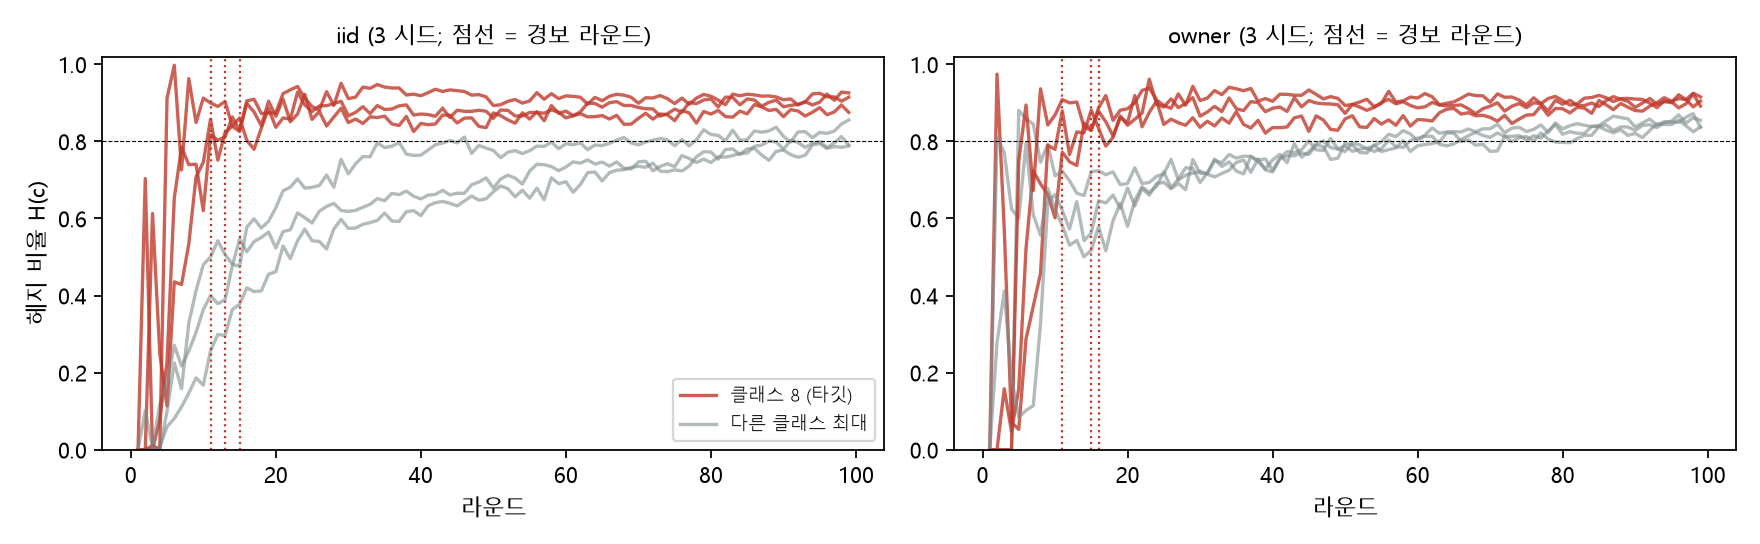
\includegraphics[width=\linewidth]{fig_H_curve.png}
\caption{라운드별 상쇄 지수 $H(c)$. 표적 클래스(적색)는 10 라운드 이내에 $h_0=0.8$을 초과하여 유지되고, 비표적 클래스의 최댓값(회색)은 그 아래에 머문다. 점선은 경보 라운드이다.}
\label{fig:H}
\end{figure}

\subsection{RQ3: 기존 계열과의 비교}
\begin{table}[t]\centering\small
\caption{기존 탐지 계열과의 비교(R-009; 동일 6 궤적, 36개 통계량 중 대표). ``검출'' = 억제자를 1순위로 지목한 시드 수. 소유자 $z$는 non-IID 조건.}
\label{tab:baselines}
\resizebox{\linewidth}{!}{%
\begin{tabular}{lccccc}\toprule
계열 (통계량) & 검출 IID · non-IID & 소유자 $z$ & 주입자 평균 순위/20 & 모델 생성 & 시점\\\midrule
업데이트 크기: 노름 · Krum · 총노출 & 3/3 · 3/3 & 3.8 · 6.8 · 2.8 & 18.5 & 없음 & 학습 중\\
업데이트 방향: 중앙값 코사인 · 반상관 · 누적 코사인 & 0/3 · 0/3 & 1.9 · 2.0 · 1.0 & 2.6--4.9 & 없음 & 학습 중\\
요청 심사 절대 변화(20\% 제거): 예측 변화 · KL & 3/3 · 3/3 & 9.7 · 65.1 & 11--15 & 요청당 단계 수 & 요청 시\\
null-space 에너지 & 1/3 · 1/3 & $-9.9$ & 3--7 & 없음 & 요청 시\\
기능 효과: 표적 집중 · Fisher & 3/3 · 3/3 & $-1.8$ · 1.7 & 8--18 & 없음 & 요청 시\\
부분 제거 상대 기준(flow $z$, 20\%) & 3/3 · 3/3 & 0.0 & 3.0--3.7 & 요청당 $K$개 & 요청 시\\
학습 중 부분합 감사(라운드 74) & 3/3 · 3/3 & 0.0 & 2.9--3.0 & 라운드당 $K$개 & 학습 중\\
참여 자연 실험(참여 회귀) & 3/3 · 3/3 & $-1.5$ & 15.0--15.2 & 없음 & 학습 중\\
\textbf{\method{}} & \textbf{3/3 · 3/3} & \textbf{배제 0/3} & \textbf{주입자 $=\mathcal{P}$ 4/4} & \textbf{없음} & \textbf{13--14 라운드}\\
\bottomrule\end{tabular}}
\end{table}
표~\ref{tab:baselines}에서 크기 기반 통계량은 억제자를 검출하지만 소유자를 함께 지목하며 주입자를 가장 정상적인 클라이언트로 평가한다. 방향 기반 통계량은 주입자가 정상 집단의 중심에 위치하여 검출에 실패한다. 절대 변화 기반 요청 심사는 소유자를 오탐한다. 억제자만을 지목하는 것은 부분 제거의 상대 기준, 기능 효과, 부분합 감사, 참여 회귀, 그리고 \method{}이며, 이 중 주입자 집합까지 식별하고 모델 생성 없이 가장 이른 시점에 동작하는 것은 \method{}뿐이다.

\subsection{RQ4: 대응}
\begin{table}[t]\centering\small
\caption{대응 기법 비교. ASR/ACC(\%), 요청자 = 억제자.}
\label{tab:remedy}
\resizebox{\linewidth}{!}{%
\begin{tabular}{llll}\toprule
기법 & IID & non-IID & 출처\\\midrule
요청자만 배제한 전체 재학습(주입자 잔존) & 44.3$\pm$23.3 / 98.8 & 29.6$\pm$19.2 / 98.4 & $K=8$ 예비(R-001 설정)\\
증류 기반 언러닝 & 18--25 / --- & --- & R-007\\
감산 + 재억제 증류 & 5.6$\pm$2.2 / 96.0$\pm$0.4 (요청자 기여 0.09 복원) & --- & R-008\\
주입자 기여의 투영 제거 & 실패 & 실패 & R-011\\
\textbf{공모 집합 배제 전체 재학습} & \textbf{0.5$\pm$0.1 / 99.0$\pm$0.0} & \textbf{0.6$\pm$0.2 / 98.9$\pm$0.0} & R-010\\
공모 집합 배제, $t_{\mathrm{back}}=13$ 복원 후 재개 & 0.68 / 99.08 (1 시드) & \todo{R-014 예정} & R-014(예비)\\
공모 집합 배제, 경보 라운드 16에서 즉시 재개 & 0.74 / 99.01 (1 시드) & \todo{R-014 예정} & R-014(예비)\\
\bottomrule\end{tabular}}
\end{table}
표~\ref{tab:remedy}는 요청자의 완전한 제거가 공격을 완성함을 보인다. 공모 집합을 배제한 경우에만 ASR 0.5\%와 ACC 99\%가 동시에 달성된다. 복원 후 재개와 경보 시점 즉시 재개는 모두 처음부터의 재학습(동일 노트북 기준 0.31\%)과 동등한 수준이며 13--16 라운드를 절약한다.

\subsection{RQ5: 매개변수 민감도}\label{sec:sens}
노트북 IID 1 시드에서 보관된 기여도로 재판정하였다(R-013). $h_0$ 0.7/0.8/0.9 $\to$ 경보 13/16/65 라운드, 식별 결과 불변. $\tau=5\to$ 22 라운드. $\kappa=1.5\to$ 정상 1명 혼입(정밀도 0.8), $\kappa=3\to$ 불변. $r=1\to$ 7 라운드에 정상 클라이언트를 억제자로 오판, $r=5\to$ 18 라운드. $\rho_0$ 1.0/0.6/0.5 $\to$ 종료 시 오경보 1/6 / 0/6 / 표적 클래스 손상 1/6. 경보 시점은 매개변수에 따라 변하나, 식별 결과는 $r\ge3$, $\kappa\ge2$, $\rho_0\in[0.6,1)$에서 불변이다.

\subsection{RQ6: 비용}
\method{}는 라운드당 9회$\times$500장의 순전파를 요구하며, 100 라운드 전체에 1--2분(노트북 GPU)이 소요된다. 요청 시점 심사(R-008)는 요청당 모델 280개 생성과 부분 제거 546회를 요구한다. 대응은 87--93 라운드의 학습으로, 처음부터의 재학습(100 라운드)보다 적다.

\section{논의 및 한계}\label{sec:limit}
\begin{itemize}
\item \textbf{오탐률.} 공격이 없는 궤적에서의 오경보율은 아직 측정되지 않았다(R-015 예정). 명제 2는 이 실측 없이는 경험적 주장으로 간주되어야 한다.
\item \textbf{전파 가정($\eta>0$).} \method{}는 상쇄가 공개 입력으로 전파되는 공격만을 관측한다. FUBA의 일관성 손실은 전파된다. BadFU의 15 라운드 궤적에서는 전파가 관측되지 않았으며(R-017, 경보 없음), 40 라운드 궤적으로 재확인한다. 전파되지 않는 경우 요청 시점의 부분 제거 심사가 보완 수단이다.
\item \textbf{복수 억제자, 다중 표적, 강건 집계.} 음의 기여 집합 규칙은 구현되어 있으나 억제자 2명 궤적에서의 실측은 예정이다. 다중 표적과 Median·Multi-Krum·FLAME·FLDetector 위의 궤적도 실측 전이다.
\item \textbf{규모.} 현재 결과는 MNIST/LeNet(FUBA 논문 설정)에 국한된다. CIFAR-10/ResNet-18 궤적은 생성 중이다.
\end{itemize}

\section{결론}
언러닝 활성화 백도어는 동일 입력 영역에 모순된 지도 신호를 공급하여 평균화로 잠복시키는 공격이며, 그 필요조건은 학습 중 클래스별 누적 기여도에 다수의 양의 기여와 단일의 음의 기여가 상쇄되는 관계적 구조로 나타난다. \method{}는 라벨·트리거·역할 정보와 모델 생성 없이 이 구조를 11--16 라운드에 검출하여 표적 클래스·억제자·주입자·복원 라운드를 산출하고, 공모 집합을 배제한 학습 재개로 삭제 요청의 이행과 백도어 제거를 동시에 달성한다.

\begin{thebibliography}{99}\small
\bibitem{zhang2023} Zhang et al. Backdoor attacks via machine unlearning (poison and mitigation samples). 2023.
\bibitem{liu2024} Liu et al. Backdoor attacks via machine unlearning. AAAI 2024.
\bibitem{ubainf} Huang et al. UBA-Inf: Unlearning activated backdoor attack with influence-driven camouflage. 2024.
\bibitem{badfu} BadFU: Backdoor federated learning through adversarial machine unlearning. 2025.
\bibitem{fuba} FUBA: Federated unlearning backdoor attack. 2025.
\bibitem{federaser} Liu et al. FedEraser: Enabling efficient client-level data removal from federated learning models. IWQoS 2021.
\bibitem{krum} Blanchard et al. Machine learning with adversaries: Byzantine tolerant gradient descent. NeurIPS 2017.
\bibitem{fltrust} Cao et al. FLTrust: Byzantine-robust federated learning via trust bootstrapping. NDSS 2021.
\bibitem{flame} Nguyen et al. FLAME: Taming backdoors in federated learning. USENIX Security 2022.
\bibitem{deepsight} Rieger et al. DeepSight: Mitigating backdoor attacks in federated learning through deep model inspection. NDSS 2022.
\bibitem{foolsgold} Fung et al. The limitations of federated learning in sybil settings. RAID 2020.
\bibitem{fldetector} Zhang et al. FLDetector: Defending federated learning against model poisoning attacks via detecting malicious clients. KDD 2022.
\bibitem{baffle} Andreina et al. BaFFLe: Backdoor detection via feedback-based federated learning. ICDCS 2021.
\bibitem{masa} MASA: Detecting malicious unlearning requests via unlearning loss. 2024.
\bibitem{subid} SubID: Subspace identification of malicious unlearning requests. INFOCOM 2026.
\bibitem{fedrecover} Cao et al. FedRecover: Recovering from poisoning attacks in federated learning using historical information. IEEE S\&P 2023.
\bibitem{hayase2022} Hayase and Oh. Few-shot backdoor attacks via neural tangent kernels. 2022.
\bibitem{koh2017} Koh and Liang. Understanding black-box predictions via influence functions. ICML 2017.
\bibitem{grabisch} Grabisch and Roubens. An axiomatic approach to the concept of interaction among players in cooperative games. Int. J. Game Theory, 1999.
\bibitem{ilharco} Ilharco et al. Editing models with task arithmetic. ICLR 2023.
\bibitem{pcgrad} Yu et al. Gradient surgery for multi-task learning. NeurIPS 2020.
\end{thebibliography}
\end{document}
